%----------------------------------------------------------------------------
%	PACKAGES AND OTHER DOCUMENT CONFIGURATIONS
%----------------------------------------------------------------------------

\documentclass[idxtotoc,hyperref,openany]{labbook}

\usepackage[ 
  backref=page,
  pdfpagelabels=true,
  plainpages=false,
  colorlinks=true,
  bookmarks=true,
  pdfview=FitB]{hyperref}
  
\usepackage{booktabs}
\usepackage{float}
\usepackage{graphicx}
\usepackage{lipsum}

\newcommand{\HRule}{\rule{\linewidth}{0.5mm}}

%----------------------------------------------------------------------------
%	DEFINITION OF EXPERIMENTS
%----------------------------------------------------------------------------

\newexperiment{PPDr}{PPD Repair After PaCE-2022}

%----------------------------------------------------------------------------

\begin{document}

%----------------------------------------------------------------------------
%	TITLE PAGE
%----------------------------------------------------------------------------

\frontmatter % Use Roman numerals for page numbers
\title{
\begin{center}
\HRule \\[0.4cm]
{\Huge \bfseries Laboratory Journal}\\[0.4cm]
\HRule \\[1.5cm]
\end{center}
}
\author{\Huge Jessica Girdwood \\ \\ \LARGE jessgirdwood@protonmail.com \\[2cm]}
\date{Beginning 20\textsuperscript{th} March 2023}
\maketitle

\tableofcontents

\mainmatter

%----------------------------------------------------------------------------
%	LAB BOOK CONTENTS
%----------------------------------------------------------------------------

\labday{20 March 2023}

\experiment{PPDr}

PPD is no longer functional after returning from a campaign in northern Finland. There are no useful images on the screen. When the trigger threshold is lowered to 10, and the trigger PMT voltage is raised above 20, there are noise triggers.

PPD was removed from its pelicase, removing and breaking the seal of the 4 bolts. The inlet heaters were disconnected, and the pump was removed. The arduino was reprogrammed to not trigger the relays. PPD was suspended above  the pelicase on two poles. The grounding point was replaced and connected to the mains socket, the mains cable was also replaced with an English plug.

\labday{21 March 2023}

\experiment{PPDr}

When the output of the trigger PMT was observed with a scope, the signal looked extremely noisy, and repeated at around \SI{5.6}{\kilo\hertz}. Figure \ref{fig:PPDScopeNoise} shows this. I was unable to determine as to whether this was the laser or the PMT, however the laser was visibly damaged so this was the suspected cause at this stage.

\begin{figure}[H]
\begin{center}
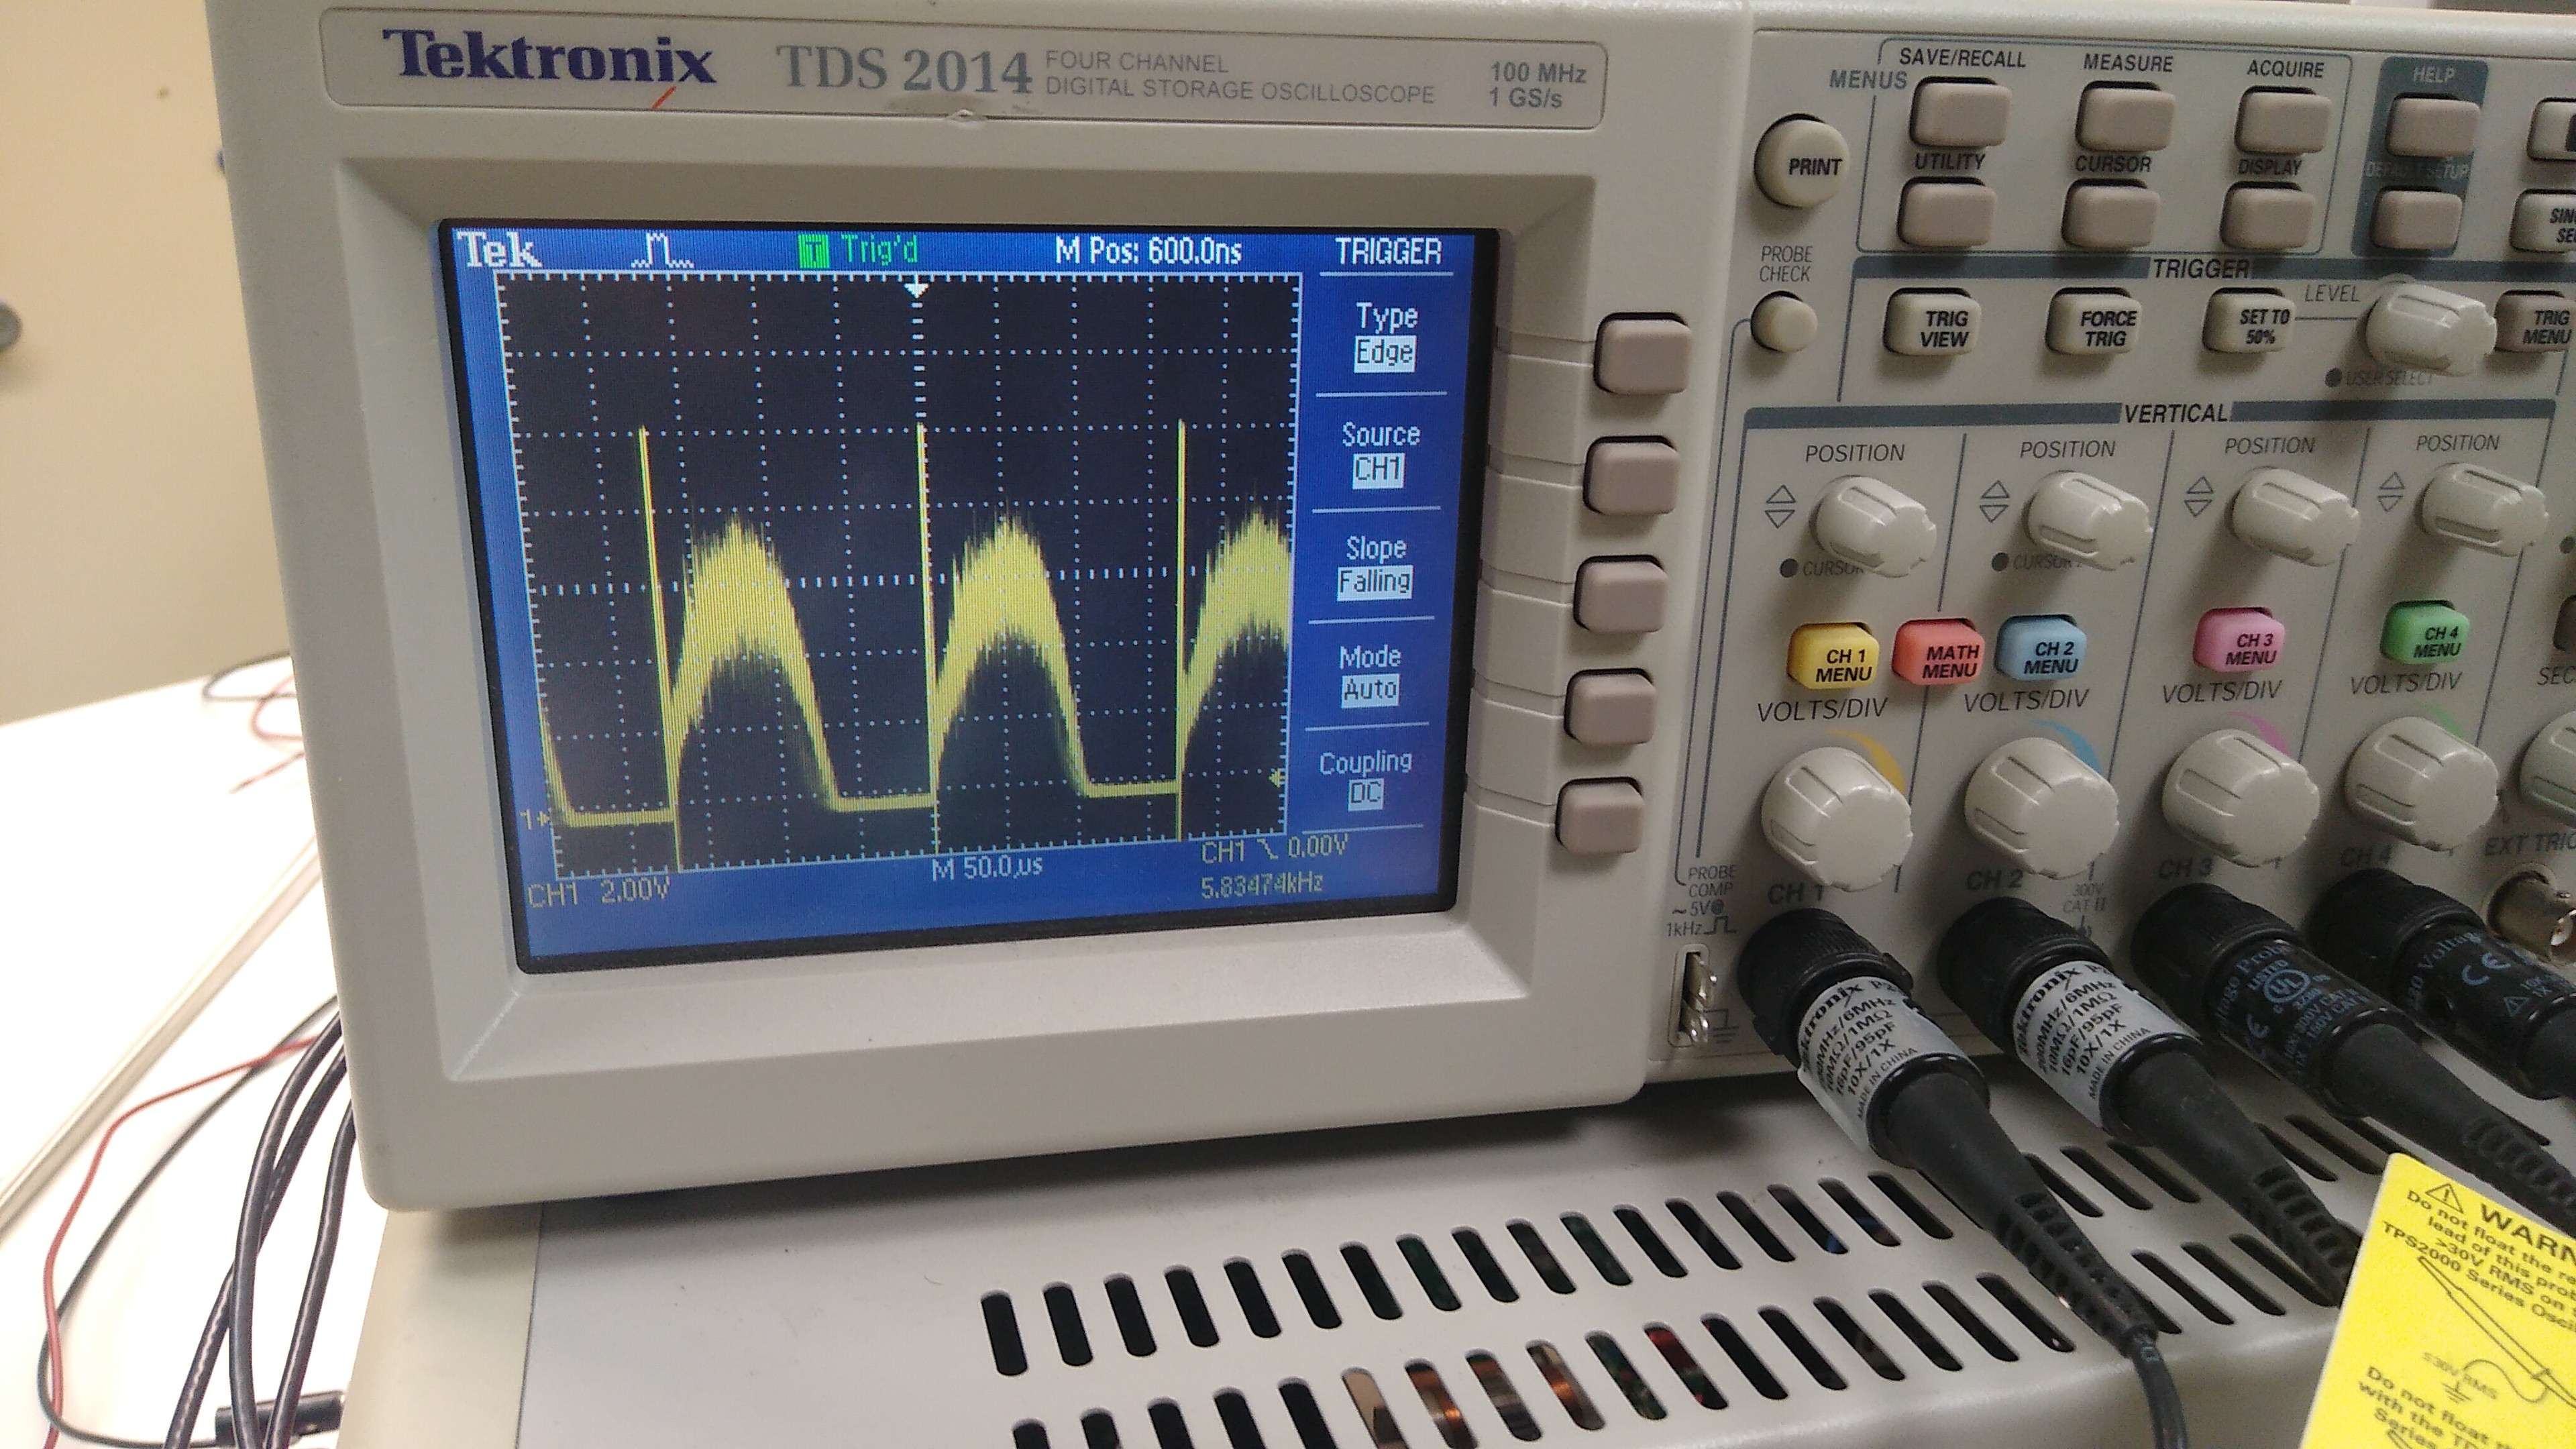
\includegraphics[width=0.5\linewidth]{Figures/PPDScopeNoise}
\end{center}
\caption{Noise after campaign with old laser.}
\label{fig:PPDScopeNoise}
\end{figure}

When an object was inserted into the optics chamber, the output resembled a square wave. This is shown in Fig. \ref{fig:PPDScatterOutput}.

\begin{figure}[H]
\begin{center}
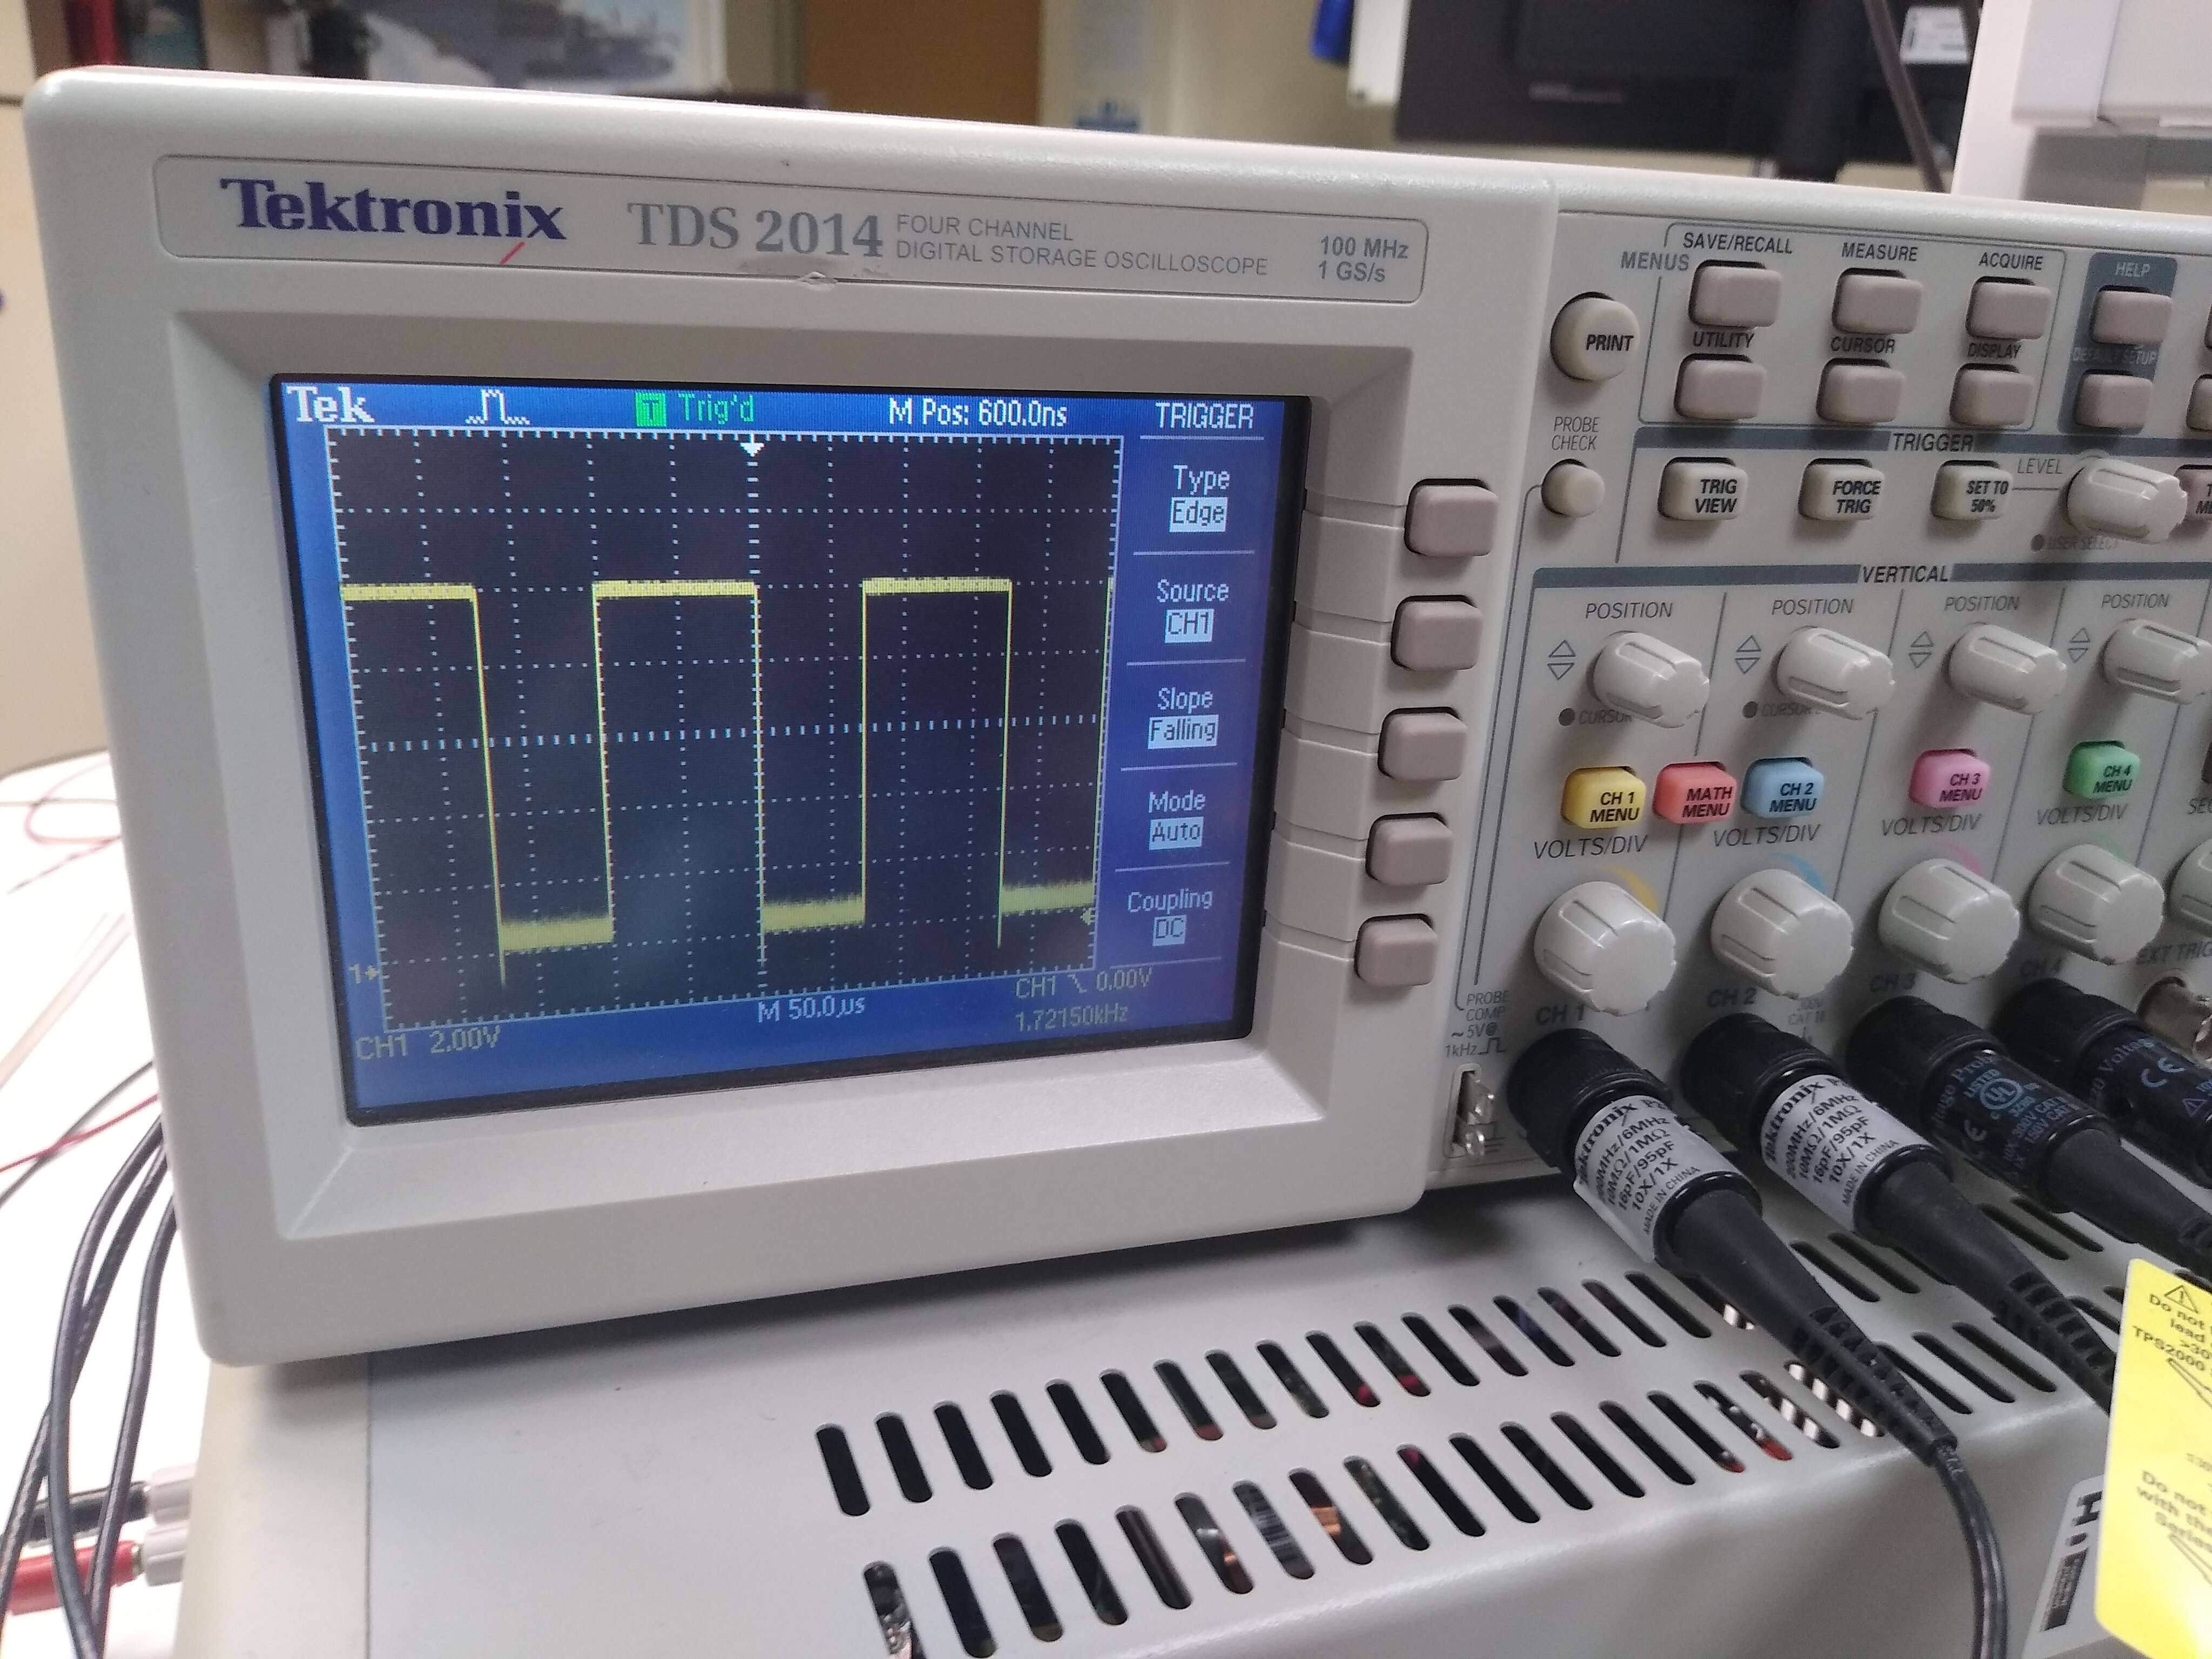
\includegraphics[width=0.5\linewidth]{Figures/PPDScatterOutput}
\end{center}
\caption{Noise after campaign with old laser and object in beam.}
\label{fig:PPDScatterOutput}
\end{figure}

The beam was also visibly dimmer, which would explain the lower image intensity. A pulse generator was configured to trigger the camera with a simulated 5 particles per second, each with a \SI{10}{\micro\second} pulse width. The camera triggering was unreliable, oftentimes exhibiting the characteristics of a "busy port".

It was decided that a new laser was the preferable option. A replacement CrystaLaser \SI{532}{\nano\metre} at \SI{150}{\milli\watt} was located.


\end{document}
















